\documentclass[9pt,twoside]{article}
\usepackage{hyperref}
\usepackage{eforms}
\usepackage{ifthen}
\usepackage[left=0.5in,top=1in,right=1in,bottom=0.75in]{geometry}
\usepackage{amsmath}
\usepackage[shortlabels]{enumitem}
\usepackage{multicol}
\usepackage{xstring}
\usepackage{fancyhdr}
\pagestyle{fancy}
\setlength{\parindent}{0in}
\usepackage[normalem]{ulem}

\usepackage{pdfpages}
\usepackage{tikz}
\usetikzlibrary{shapes.misc,shadows}

\newcommand{\IfStringInList}[2]{\IfSubStr{,#2,}{,#1,}}

\newcommand{\textovaled}[1]{%
\begin{tikzpicture}[baseline=(char.base)]
\node(char)[draw,fill=white,
  shape=rounded rectangle,
%  drop shadow={opacity=.5,shadow xshift=0pt},
  minimum width=1.8cm]
  {#1};
\end{tikzpicture}%
}



\provideboolean{include-CV}

\newcommand{\thesissubmissiondate}{(not yet submitted)}%September 18, 2020}


\bgroup

\def\title{\gdef\thesistitle}
\def\author{\gdef\authorname}
\def\department{\gdef\department}
\def\degree{\gdef\degree}
\def\degreemonth{\gdef\degreemonth}
\def\degreeyear{\gdef\degreeyear}
\def\thesisdate{\gdef\thesisdate}
\def\chairman#1#2{\gdef\chairman{{#1}{#2}}}

\title{Performance Engineering of Proof-Based Software Systems}
% Alternative (kind-of joke) title: Coq Performance Issues
% Alternative alternative joke title: How To Avoid Hen Performance Issues
% (hen, because people are ``too obsessed with Coq performance'', so we'll have to name our next proof assistant after hens rather than roosters)

\author{Jason S.~Gross}
% If you wish to list your previous degrees on the cover page, use the
% previous degrees command:
%       \prevdegrees{A.A., Harvard University (1985)}
% You can use the \\ command to list multiple previous degrees
%       \prevdegrees{B.S., University of California (1978) \\
%                    S.M., Massachusetts Institute of Technology (1981)}
\department{Department of Electrical Engineering and Computer Science}

% If the thesis is for two degrees simultaneously, list them both
% separated by \and like this:
% \degree{Doctor of Philosophy \and Master of Science}
\degree{Doctor of Philosophy in Computer Science and Engineering}

% As of the 2007-08 academic year, valid degree months are September,
% February, or June.  The default is June.
\degreemonth{February}
\degreeyear{2021}
\thesisdate{(draft)}%August 19, 2015}


%% By default, the thesis will be copyrighted to MIT.  If you need to copyright
%% the thesis to yourself, just specify the `vi' documentclass option.  If for
%% some reason you want to exactly specify the copyright notice text, you can
%% use the \copyrightnoticetext command.
%\copyrightnoticetext{\copyright IBM, 1990.  Do not open till Xmas.}

% This is the department committee chairman, not the thesis committee
% chairman.  You should replace this with your Department's Committee
% Chairman.
\chairman{Leslie A.~Kolodziejski}{Chair, Department Committee on Graduate Students}
\todo{Is the ``department committee chairman'' still Leslie A. Kolodziejski?}

\todo{make sure author and title show up in pdf info}


\egroup

\def\citizenship{United States}
\def\area{EE}
\def\supervisor{Adam Chlipala}
\def\degreelistdate{\degreemonth\space \degreeyear}
\def\newinstitution{}
\def\newtitle{}
\def\newlocation{}
\def\typeofjob{Industry}
\def\otherjob{}
\def\employmentarea{Programming Language/Compilers}
\def\otheremployment{}

\newcommand{\checkTypeOfJob}[1]{%
  \IfStringInList{#1}{\typeofjob}{\def\typeV{\V{Yes}}}{\def\typeV{}}%
  \expandafter\checkBox\expandafter[\typeV]{type of job: #1}{\baselineskip}{\baselineskip}{Yes} #1%
}

\newcommand{\checkOtherJob}{%
  \ifthenelse{\equal{\otherjob}{}}{\def\typeV{}}{\def\typeV{\V{Yes}}}%
  \expandafter\checkBox\expandafter[\typeV]{type of job: Other}{\baselineskip}{\baselineskip}{Yes} Other \\
  \expandafter\checkBox\expandafter[\typeV]{type of job: Other}{\baselineskip}{\baselineskip}{Yes}\ \textField[\V{\otherjob}]{other job}{15em}{\baselineskip}
}

\newcommand{\checkEmploymentArea}[1]{%
  \IfStringInList{#1}{\employmentarea}{\def\employmentV{\V{Yes}}}{\def\employmentV{}}%
  \expandafter\checkBox\expandafter[\employmentV]{area of employment: #1}{\baselineskip}{\baselineskip}{Yes} #1%
}

\newcommand{\checkOtherEmployment}{%
  \ifthenelse{\equal{\otheremployment}{}}{\def\employmentV{}}{\def\employmentV{\V{Yes}}}%
  \expandafter\checkBox\expandafter[\employmentV]{area of employment: Other}{\baselineskip}{\baselineskip}{Yes} Other: \\
  \expandafter\checkBox\expandafter[\employmentV]{area of employment: Other}{\baselineskip}{\baselineskip}{Yes}\ \textField[\V{\otheremployment}]{other employment}{15em}{\baselineskip}
}

\begin{document}
\lhead{\textbf{PHD/SCD COMPLETION FORM}}
\rhead{\textbf{2020-2021}}
\cfoot{}
\renewcommand{\headrulewidth}{0pt}
\everyTextField{\BC{}}

This form is to be completed by EECS graduate students upon submission of a doctoral thesis to the
department. \textbf{Please attach a CV or resume\ldots{}thank you.}

\fbox{\begin{minipage}{\textwidth}
{\Large STUDENT NAME:\ \textField[\V{\authorname}]{name}{\textwidth-\widthof{STUDENT NAME:\ }}{\baselineskip}} \\
\\
\newlength{\realbaselineskip}%
\setlength{\realbaselineskip}{\baselineskip}%
\begin{tabular}{lll}
CITIZENSHIP (circle) \qquad
 & {\ifthenelse{\equal{\citizenship}{United States}}{%
     }{%
       \def\textovaled{}%
     }%
     \textovaled{United States}%
   } \qquad
  & {\ifthenelse{\equal{\citizenship}{United States}}{%
        \def\citizenship{}%
        \def\textovaled{}%
      }{}%
      \textovaled{OTHER: \textField[\V{\citizenship}]{citizenship}{\widthof{United States of America of America}}{\realbaselineskip}}} \\ \\
AREA (circle):
& {\ifthenelse{\equal{\area}{EE}}{}{\def\textovaled{}}%
    \textovaled{\fbox{EE}}} \hfill \textbf{or}
& {\ifthenelse{\equal{\area}{CS}}{}{\def\textovaled{}}%
    \textovaled{\fbox{CS}}} \\ \\
\multicolumn{3}{l}{%
  DATE of THESIS SUBMISSION:\ \textField[\V{\thesissubmissiondate}]{thesis submission date}{25em}{\realbaselineskip}%
} \\ \\
\multicolumn{3}{l}{%
  THESIS SUPERVISOR(S):\ \textField[\V{\supervisor}]{supervisor}{\textwidth-\widthof{THESIS SUPERVISOR(S):\ }-2em}{\realbaselineskip}%
} \\ \\
\multicolumn{3}{l}{%
  DATE of MIT DEGREE LIST:\ \textField[\V{\degreelistdate}]{MIT degree list date}{25em}{\realbaselineskip}%
}
\end{tabular}
\end{minipage}}
$\left.\right.$ \\ \\
\uline{Please notify us of your immediate future plans, by responding to the questions below:}

\begin{enumerate}
  \item
    Please check the type of job you are taking within the following broad categories:
    \begin{multicols}{2}
      \checkTypeOfJob{Academic/faculty position} \\
      \checkTypeOfJob{Academic/researcher} \\
      \checkTypeOfJob{Academic/postdoc} \\
      \checkTypeOfJob{Industry} \\
      \checkTypeOfJob{Government} \\
      \checkTypeOfJob{Medical} \\
      \columnbreak \\
      \checkTypeOfJob{Financial} \\
      \checkTypeOfJob{Management Consulting} \\
      \checkTypeOfJob{Self-Employed} \\
      \checkOtherJob{} \\
      \checkTypeOfJob{Un-Employed} \\
    \end{multicols}
  \item $\left.\right.$\\
    \raisebox{\baselineskip}{\fbox{\begin{minipage}{\textwidth-5em}
        If you can let us know specifically where you are going, that would be most helpful: \\ \\
        Institution:\ \textField[\V{\newinstitution}]{institution}{\textwidth-3em-\widthof{Institution:\ }}{\baselineskip} \\ \\
        Title:\ \textField[\V{\newtitle}]{title}{\textwidth-3em-\widthof{Title:\ }}{\baselineskip} \\ \\
        Location of Employment:\ \textField[\V{\newlocation}]{location of employment}{\textwidth-3em-\widthof{Location Of Employment:\ }}{\baselineskip} \\
      \end{minipage}}}
  \item
    Check the area within EECS that best describes your area of employment:
    \begin{multicols}{2}
      \checkEmploymentArea{Communications} \\
      \checkEmploymentArea{Systems, Decision and Control} \\
      \checkEmploymentArea{Signal Processing} \\
      \checkEmploymentArea{Bioelectrical/Medical Engineering} \\
      \checkEmploymentArea{Circuit Design} \\
      \checkEmploymentArea{Devices and Materials} \\
      \checkEmploymentArea{Electromagnetics and Energy} \\
      \checkEmploymentArea{Artificial Intelligence/Robotics} \\
      \columnbreak \\
      \checkEmploymentArea{Hardware/ Architecture} \\
      \checkEmploymentArea{Numerical Analysis/Scientific} \\
      \checkEmploymentArea{Programming Language/Compilers} \\
      \checkEmploymentArea{OS/Networks} \\
      \checkEmploymentArea{Software Engineering} \\
      \checkEmploymentArea{Theory/ Algorithms} \\
      \checkEmploymentArea{Graphics/Human Interface} \\
      \checkEmploymentArea{Database/Information Systems} \\
      \checkOtherEmployment{} \\
    \end{multicols}
\end{enumerate}
\begin{center}
  \textbf{THANK YOU, and ALL GOOD WISHES!}
\end{center}
\clearpage
\fancyhf{}
\ifthenelse{\boolean{include-CV}}{%
  \cleardoublepage
  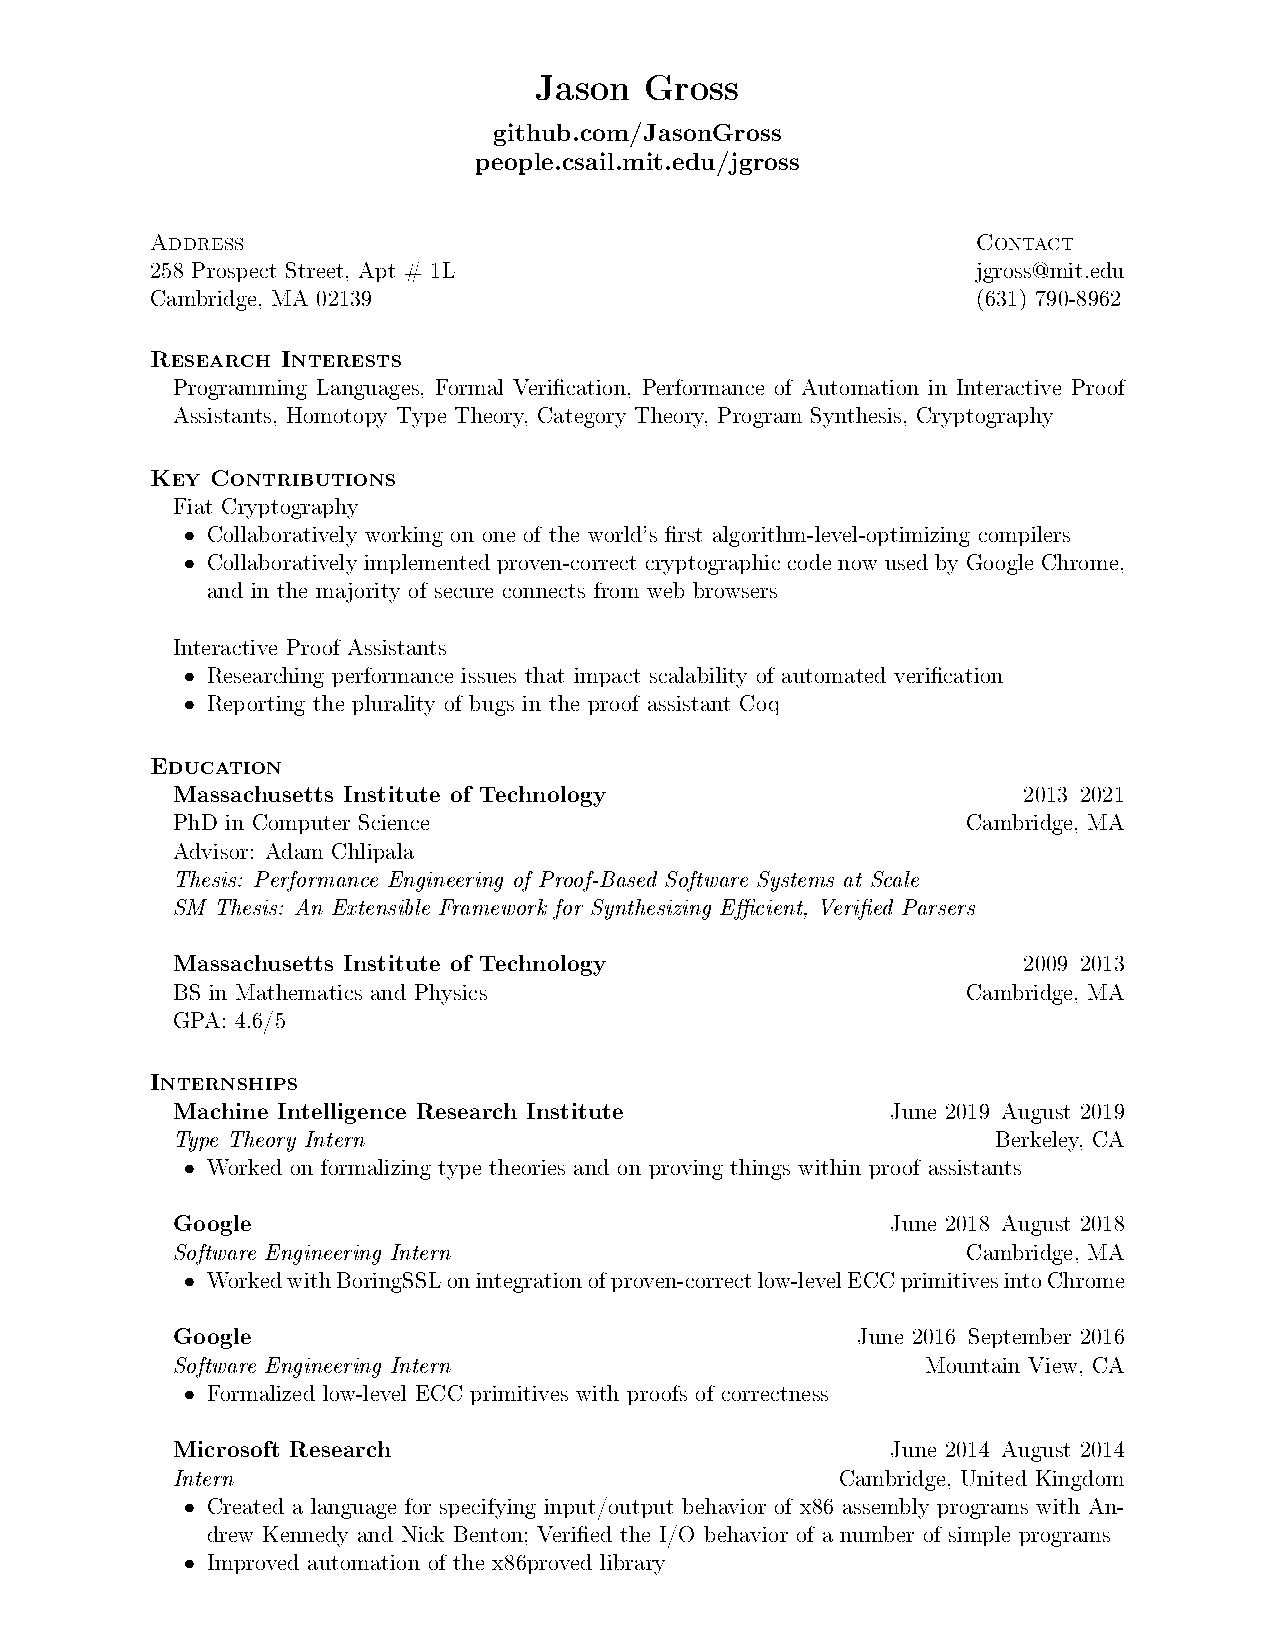
\includepdf[pages={1-}]{resume/Resume-curriculum-vitae}
}{%
}
\end{document}
